\documentclass[10pt]{article}
\usepackage[portuguese]{babel}
\usepackage[a4paper, top = 0.8in, bottom = 0.9in, left =0.6in, right = 0.6in]{geometry}
\usepackage{inputenc}
\usepackage{fancyhdr}
\usepackage{multirow}
\usepackage{graphicx}
\usepackage{times}
\usepackage{subcaption}
\usepackage{booktabs}
\usepackage{microtype}
\usepackage{wrapfig}
\usepackage{circuitikz}
\usepackage{titlesec}
\usepackage{wrapfig}
\usepackage{listings}
\usepackage{tikz}

\usepackage{caption}
\usepackage{ragged2e}
\usepackage{adjustbox}
\usepackage{float}
\usepackage{amsmath, mathtools, amssymb}
\usepackage{parskip}
\usepackage{array, makecell}
\usepackage{booktabs}
\titleformat{\section}
{\normalfont\large\bfseries}{\thesection)}{1em}{}
\titleformat{\subsection}
{\normalfont\normalsize\bfseries}{\thesubsection)}{1em}{}
\titleformat{\subsubsection}
{\normalfont\normalsize\bfseries}{\thesubsubsection)}{1em}{}


%\pretitle{\begin{center}\Huge\bfseries}

\pagestyle{fancy}
\fancyhead{}
\centering\chead{
\includegraphics[width=15cm]{imagens/unb_fga_logo_extenso.jpg}}
\lfoot{Prática de Circuitos 1 - 2020/1}
\rfoot{\textbf{Prof. Dr. Marcus V. Chaffim Costa}} %nome do rodape
\renewcommand{\footrulewidth}{1pt}

\setlength{\parskip}{0.1cm}
\author{Monitoria - 2019/2}
\title{Tutorial 10}


%arrumação das tabelas

\setlength{\tabcolsep}{0.5em} % for the horizontal padding
{\renewcommand{\arraystretch}{1.2}}% for the vertical padding
\captionsetup[table]{name= \bfseries Tabela}
\numberwithin{table}{section}
\usepackage{array}
\newcolumntype{C}[1]{>{\centering\arraybackslash}m{#1}}

\aboverulesep=0cm
\belowrulesep=0cm

%configuracoes dos codigos em matlab

\usepackage{color} %red, green, blue, yellow, cyan, magenta, black, white
\definecolor{mygreen}{RGB}{28,172,0} % color values Red, Green, Blue
\definecolor{mylilas}{RGB}{170,55,241}

\lstset{language=Matlab,%
    %basicstyle=\color{red},
    breaklines=true,%
    morekeywords={matlab2tikz},
    keywordstyle=\color{blue},%
    morekeywords=[2]{1}, keywordstyle=[2]{\color{black}},
    identifierstyle=\color{black},%
    stringstyle=\color{mylilas},
    commentstyle=\color{mygreen},%
    showstringspaces=false,%without this there will be a symbol in the places where there is a space
    numbers=left,%
    numberstyle={\tiny \color{black}},% size of the numbers
    numbersep=9pt, % this defines how far the numbers are from the text
    emph=[1]{for,end,break},emphstyle=[1]\color{red}, %some words to emphasise
    %emph=[2]{word1,word2}, emphstyle=[2]{style},    
}

\allowdisplaybreaks


%==============macros para uso nos documentos===================%

\newcommand{\ohm}{\Omega}


\newcommand{\figuras}[4]{
    \begin{figure}[H]
        \centering
        \includegraphics[width={#1}\textwidth]{{#2}}
        \caption{{#3}}
        \label{fig:{#4}}
    \end{figure}
}

\newcommand{\figura}[2]{
    \begin{figure}[H]
        \centering
        \includegraphics[width={#1}\textwidth]{{#2}}
    \end{figure}
}

\newcommand{\subfiguras}[5]{
    \centering
    \begin{subfigure}[H]{#1\textwidth}
        \centering
        \includegraphics[width={#2}\textwidth]{{#3}}
        \caption{{#4}}
        \label{fig:{#5}}
    \end{subfigure}
}

\newcommand{\circuito}[3]{
    \begin{figure}[H]
        \centering
        \begin{circuitikz}[line width=.5pt]
            #1
        \end{circuitikz}
        \caption{{#2}}
        \label{circ:{#3}}    
    \end{figure}
}

\newcommand{\calc}[1]{
    \begin{gather*}
        #1
    \end{gather*}
}





%=====================================================%

\usetikzlibrary{automata}

\begin{document}

\begin{center}
\vspace*{.03cm}
\Large\bfseries{Experimento 10:}\\ %titulo
\Large{Integrador e Diferenciador com Amplificador Operacional}
\end{center}
\justify

\section{Estudo pré-laboratorial}
\subsection{Princípio da Superposição e Conversores D/A}


Os sinais elétricos podem ser descritos genericamente como estando nas formas analógica ou digital. Um sinal analógico é contínuo tanto no tempo quanto na amplitude. Como exemplo, pode-se citar um sinal de uma gravação de música na saída de um amplificador de áudio que alimenta um alto-falante. Por outro lado, um sinal digital, tipicamente representado por números binários, corresponde a uma representação por amostras do sinal analógico original. As amostras do sinal digital podem assumir valores discretos (isto é, um número finito de valores) e representam o sinal em instantes de tempo discretos (em instantes de tempo definidos). Assim, um número binário pode corresponder a um determinado valor de tensão em um determinado instante de tempo. A Fig. 2.1 ilustra o processo de digitalização de um sinal de áudio. Primeiramente, os valores de tensão do sinal analógico (Fig. 2.1a) são tomados a intervalos regulares de tempo, resultando no sinal amostrado (Fig. 2.1b). Depois, o sinal amostrado é quantizado (Fig. 2.1c), ou seja, cada valor de tensão do sinal amostrado será substituído por um dos 2n valores de tensão possíveis, onde n é o número de bits que irão representar cada amostra. Por fim, o sinal quantizado é convertido em uma sequência de bits, onde cada grupo de bits corresponde a um dos valores possíveis no processo de quantização (Fig. 2.1d). Um problema importante em engenharia eletrônica é o uso de um circuito para a conversão de um sinal da forma digital para a forma analógica. O circuito poderia ser usado, por exemplo, em um aparelho de CD. Um número binário (formado por zeros e uns) — correspondente a uma amostra do sinal original, gravado no CD — deve ser convertido para um valor de tensão, que vai representar uma aproximação do sinal analógico durante um intervalo de tempo definido. Um circuito para converter de digital para analógico é apresentado na Fig. 2.2. Cada um dos bits do número binário está associado a um conjunto formado por uma bateria e uma chave. Quando o valor do bit é igual a 1 , a chave correspondente é conectada à bateria; quando o valor é igual a 0 , a chave é conectada ao terra do circuito. A posição da chave é controlada pelo valor do bit. Desta forma, um número binário 000 faz aparecer uma tensão V o = 0 V , enquanto que o número 111 faz aparecer uma tensão V o = 7 / 12 V bat . No circuito, cada número binário entre 000 e 111 corresponde a um valor de tensão que vai representar uma amostra do sinal durante um intervalo de tempo determinado. Por exemplo, para obter uma forma de onda do tipo rampa na saída V o , bastaria escrever em sequência as palavras binárias que vão de 000 a 111 , em incrementos de 1 . Um conversor D/A com mais bits pode ser obtido simplesmente acrescentando novos pares de resistores R-2R e novas chaves ao circuito.
\begin{figure}[H] 
  \centering 
  \begin{subfigure}{.33\textwidth}
    \centering
    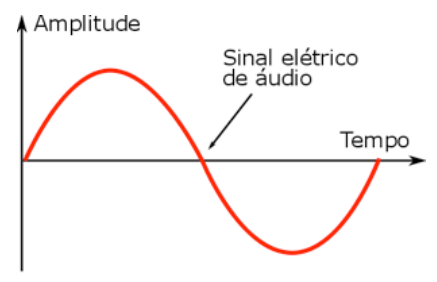
\includegraphics[width=.5\textwidth]{imagens/pdf_images/a.png}
    \caption{}
    \label{fig:a_sf}
  \end{subfigure}
  \begin{subfigure}{.33\textwidth}
    \centering
    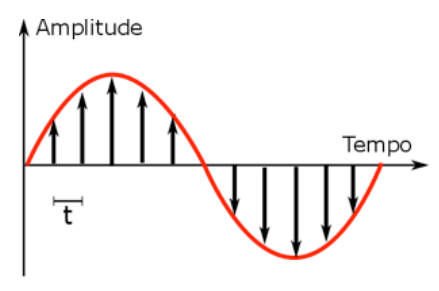
\includegraphics[width=.5\textwidth]{imagens/pdf_images/b.png}
    \caption{}
    \label{fig:b_sf}
  \end{subfigure}
  \begin{subfigure}{.33\textwidth}
    \centering
    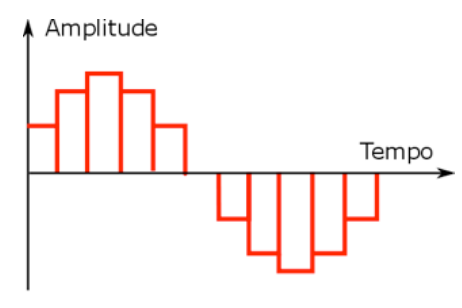
\includegraphics[width=.5\textwidth]{imagens/pdf_images/c.png}
    \caption{}
    \label{fig:c_sf}
  \end{subfigure}
  
  \begin{subfigure}{.33\textwidth}
    \centering
    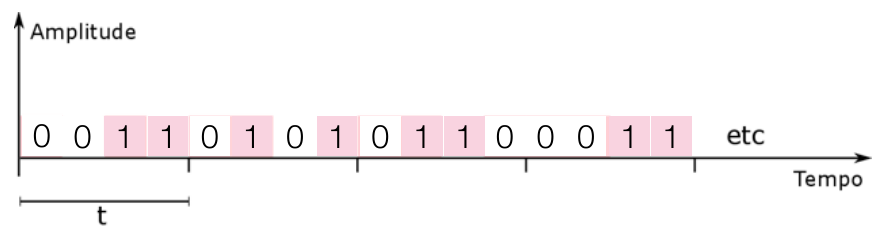
\includegraphics[width=1.3\textwidth]{imagens/pdf_images/d.png}
    \caption{}
    \label{fig:d_sf}
  \end{subfigure}
  
  
  \caption{Conversão analógico-digital (A/D): (a) sinal analógico; (b) discretização no tempo (amostragem); (c) discretização em amplitude (quantização); e (d) representação do sinal digital na forma de bits.}
  \label{fig:fig1}
\end{figure}

\begin{figure}[H]
  \centering
  \begin{circuitikz}[line width = .5pt, scale = .8, transform shape, american voltages]
    \draw
      (0,0) node [ground] {} -- (0,.5)
      to [short] (5,.5) to [R,l=$2R$] (5,8) -- (3,8)
      to [R,l=$R$, *-] (0,8) to [R,l=$R$, *-*] (-3,8) -- (-5,8) -- (-5,5)
      to [R, l=$2R$, v=$V_o$] (-5, 3) -- (-5,.5) -- (0,.5);
    \draw
    (-3,8) to [R,l=$2R$] (-3,5.5);
    \draw
    (-3,5)  node [spdt, rotate = -90] (Sw){}
    (Sw.out 2) to [short, -*] ($(Sw.out 2)-(0,3.9)$); 
    \draw
    (-2.5,5) node [right] {bit2};
    \draw
    (3,5)  node [spdt, rotate = -90] (Sw3){}
    (Sw3.out 1) to [short, -*] ($(Sw3.out 1)-(0,3.9)$); 
    \draw
    (3,8) to [R, l=$2R$] (3,5.5); 
    \draw
    ($(Sw.out 1) - (0,.5)$) -- ($(Sw3.out 2)-(0,.5)$);
    \draw
    (Sw.out 1) -- ($(Sw.out 1) - (0,.5)$) to [short, -*] (.3,3.9) -- 
    ($(Sw3.out 2) - (0,.5)$)--(Sw3.out 2);
    \draw
    (0,8) to [R, l=$2R$] (0,5.5);
    \draw
    (0,5) node [spdt, rotate = -90] (Sw2) {};
    \draw
    (1.5,5) node [left] {bit1};
    \draw 
    (.3,.5) to [battery, v_<=$Vbat$, *-]  (Sw2.out 1);
    \draw
    (Sw2.out 2) -- ($(Sw2.out 2) -(.5,0)$) -- (-.8,.5);
    \draw
    (4.5,5) node [left] {bit0};
    
  \end{circuitikz}
  \caption{Conversor Digital-Analógico (D/A) tipo rede R-2R de 3 bits.}
  \label{circ:conv_da}
\end{figure}

\subsubsection{Por meio de análise teórica do circuito da Fig. 2.2, encontre o valor da saída V o para cada uma das 8 palavras binárias de 3 bits possíveis ( 000 a 111 ). Para tal, considere $V_{bat}$ = 5 V.}


\noindent Dica: ao invés de resolver o circuito oito vezes, resolva apenas para as palavras binárias 000, 001, 010 e 100. A seguir, aplique o teorema da superposição para encontrar o resultado para as demais palavras binárias 


\noindent \textbf{a)} Para a palavra binária 000, tem-se o seguinte circuito:


\begin{figure}[H]
  \centering
  \begin{circuitikz}[line width = .5pt, scale = .8, transform shape, american voltages]
    \draw
      (0,0) node [ground] {} -- (0,.5)
      to [short] (5,.5) to [R,l=$2R$] (5,8) -- (3,8)
      to [R,l=$R$, *-] (0,8) to [R,l=$R$, *-*] (-3,8) -- (-5,8) -- (-5,5)
      to [R, l=$2R$, v=$V_o$] (-5, 3) -- (-5,.5) -- (0,.5);
    \draw
    (-3,8) node [above, color=red] {A} to [R,l=$2R$] (-3,5.5);
    \draw
    (-3,5)  node [spdt, rotate = 90, xscale=-1] (Sw){}
    (Sw.out 1) to [short, -*] ($(Sw.out 1)-(0,3.9)$); 
    \draw
    (-2.5,5) node [right] {bit2};
    \draw
    (3,5)  node [spdt, rotate =-90, xscale=1] (Sw3){}
    (Sw3.out 1) to [short, -*] ($(Sw3.out 1)-(0,3.9)$); 
    \draw
    (3,8) node [above, color=red] {C} to [R, l=$2R$] (3,5.5); 
    \draw 
    (Sw.out 2) -- ($(Sw.out 2) - (0,.5)$) to [short, -*] (.3,3.9) -- 
    ($(Sw3.out 2) - (0,.5)$)--(Sw3.out 2);
    \draw
    (0,8) node [above, color=red] {B} to [R, l=$2R$] (0,5.5);
    \draw
    (0,5) node [spdt, rotate = 90, xscale=-1] (Sw2) {};
    \draw
    (1.5,5) node [left] {bit1};
    \draw 
    (.3,.5) to [battery, v_<=$Vbat$, *-]  (Sw2.out 2);
    \draw
    (Sw2.out 1) -- ($(Sw2.out 1) -(.5,0)$) -- (-.8,.5);
    \draw
    (4.5,5) node [left] {bit0};
    
  \end{circuitikz}
  \caption{Conversor Digital-Analógico (D/A) tipo rede R-2R de 3 bits.}
  \label{circ:conv_da}
\end{figure}


Como não há participação da fonte (bateria), então o valor de $V_o=V_{000}=0V$.

\textbf{b)} Para a palavra binária 001, tem-se o seguinte resultado:

\begin{figure}[H]
  \centering
  \begin{circuitikz}[line width = .5pt, scale = .8, transform shape, american voltages]
    \draw
      (0,0) node [ground] {} -- (0,.5)
      to [short] (5,.5) to [R,l=$2R$] (5,8) -- (3,8)
      to [R,l=$R$, *-] (0,8) to [R,l=$R$, *-*] (-3,8) -- (-5,8) -- (-5,5)
      to [R, l=$2R$, v=$V_o$] (-5, 3) -- (-5,.5) -- (0,.5);
    \draw
    (-3,8) node [above, color=red] {A} to [R,l=$2R$] (-3,5.5);
    \draw
    (-3,5)  node [spdt, rotate = 90, xscale=-1] (Sw){}
    (Sw.out 1) to [short, -*] ($(Sw.out 1)-(0,3.9)$); 
    \draw
    (-2.5,5) node [right] {bit2};
    \draw
    (3,5)  node [spdt, rotate =90, xscale=-1] (Sw3){}
    (Sw3.out 2) to [short, -*] ($(Sw3.out 2)-(0,3.9)$); 
    \draw
    (3,8) node [above, color=red] {C} to [R, l=$2R$] (3,5.5); 
    \draw 
    (Sw.out 2) -- ($(Sw.out 2) - (0,.5)$) to [short, -*] (.3,3.9) -- 
    ($(Sw3.out 1) - (0,.5)$)--(Sw3.out 1);
    \draw
    (0,8) node [above, color=red] {B} to [R, l=$2R$] (0,5.5);
    \draw
    (0,5) node [spdt, rotate = 90, xscale=-1] (Sw2) {};
    \draw
    (1.5,5) node [left] {bit1};
    \draw 
    (.3,.5) to [battery, v_<=$Vbat$, *-]  (Sw2.out 2);
    \draw
    (Sw2.out 1) -- ($(Sw2.out 1) -(.5,0)$) -- (-.8,.5);
    \draw
    (4.5,5) node [left] {bit0};
    
  \end{circuitikz}
  \caption{Conversor Digital-Analógico (D/A) tipo rede R-2R de 3 bits.}
  \label{circ:conv_da}
\end{figure}

Aplicando a LKT, temos
\[
\begin{cases}
  \dfrac{V_A - V_B}{R} + \dfrac{V_A}{2R}=0\\
  \\
  \dfrac{V_B - V_A}{R} + \dfrac{V_B}{2R} + \dfrac{V_B - V_C}{R}=0\\
  \\
  \dfrac{V_C - V_B}{R} + \dfrac{V_C - 5}{2R} + \dfrac{V_C}{2R}=0
\end{cases}
\rightarrow
\begin{cases}
  2V_A-V_B+0V_C=0\\
  -1V_A + 2,5V_B-1V_C=0\\
  0V_A-1V_b+2V_C=0
\end{cases}
\]

Transpondo o sistema de equações obtido acima para uma matriz $3x3$, temos

\[
\begin{bmatrix}
  2 & -1 & 0\\
  -1 & 2,5 & -1\\
  0 & -1 & 2
\end{bmatrix}
\cdot
\begin{bmatrix}
  V_A\\
  V_B\\
  V_C
\end{bmatrix}
=
\begin{bmatrix}
  0\\0\\0
\end{bmatrix}
\]

Resolvendo a matriz encontramos
\[
  \begin{cases}
    V_A=0,4167\\V_B=0,8333\\V_C=1,6667
  \end{cases}
\]

Logo, 

\begin{equation}
  V_A=V_o=V_{001}=0,4167V
\end{equation}

\textbf{c)} Para a palavra binária 010, temos a seguinte configuração


\begin{figure}[H]
  \centering
  \begin{circuitikz}[line width = .5pt, scale = .8, transform shape, american voltages]
    \draw
      (0,0) node [ground] {} -- (0,.5)
      to [short] (5,.5) to [R,l=$2R$] (5,8) -- (3,8)
      to [R,l=$R$, *-] (0,8) to [R,l=$R$, *-*] (-3,8) -- (-5,8) -- (-5,5)
      to [R, l=$2R$, v=$V_o$] (-5, 3) -- (-5,.5) -- (0,.5);
    \draw
    (-3,8) node [above, color=red] {A} to [R,l=$2R$] (-3,5.5);
    \draw
    (-3,5)  node [spdt, rotate = 90, xscale=-1] (Sw){}
    (Sw.out 1) to [short, -*] ($(Sw.out 1)-(0,3.9)$); 
    \draw
    (-2.5,5) node [right] {bit2};
    \draw
    (3,5)  node [spdt, rotate =-90, xscale=1] (Sw3){}
    (Sw3.out 1) to [short, -*] ($(Sw3.out 1)-(0,3.9)$); 
    \draw
    (3,8) node [above, color=red] {C} to [R, l=$2R$] (3,5.5); 
    \draw 
    (Sw.out 2) -- ($(Sw.out 2) - (0,.5)$) to [short, -*] (.3,3.9) -- 
    ($(Sw3.out 2) - (0,.5)$)--(Sw3.out 2);
    \draw
    (0,8) node [above, color=red] {B} to [R, l=$2R$] (0,5.5);
    \draw
    (0,5) node [spdt, rotate =-90, xscale=1] (Sw2) {};
    \draw
    (1.5,5) node [left] {bit1};
    \draw 
    (.3,.5) to [battery, v_<=$Vbat$, *-]  (Sw2.out 1);
    \draw
    (Sw2.out 2) -- ($(Sw2.out 2) -(.5,0)$) -- (-.8,.5);
    \draw
    (4.5,5) node [left] {bit0};
    
  \end{circuitikz}
  \caption{Conversor Digital-Analógico (D/A) tipo rede R-2R de 3 bits.}
  \label{circ:conv_da}
\end{figure}

Aplicando a LKT, temos

\[
  \begin{cases}
    \dfrac{V_A - V_B}{R} + \dfrac{V_A}{2R} + \dfrac{V_A}{2R} =0\\
    \\
    \dfrac{V_B - V_A}{R} + \dfrac{V_B - 5}{2R} + \dfrac{V_B - V_C}{R}  =0\\
    \\
    \dfrac{V_C - V_B}{R} + \dfrac{V_C}{2R} + \dfrac{V_C}{2R} =0
  \end{cases}
  \rightarrow
  \begin{cases}
    2V_A - 1V_B + 0V_C = 0  \\
    -1V_A + 2,5V_B - 1V_C=2,5\\
    0V_A-1V_B+2V_C=0
  \end{cases}
\]

Colocando em forma matricial, tem-se

\[
  \begin{bmatrix}
    2 & -1 & 0\\
    -1 & 2,5 & -1 \\
    0 & -1 & 2
  \end{bmatrix}
  \cdot 
  \begin{bmatrix}
    V_A\\V_B\\V_C
  \end{bmatrix}
  =
  \begin{bmatrix}
    0\\2,5\\0
  \end{bmatrix}
\]

Resolvendo a matriz, obtem-se

\[
  \begin{cases}
    V_A=0,8333V\\V_B=1,6667V\\V_C=0,8333V
  \end{cases}
\]
Logo,

\begin{equation}
  V_A=V_o=V_{010}=0,8333V
\end{equation}

\textbf{d)} Para a palavra 100, tem-se o seguinte circuito


\begin{figure}[H]
  \centering
  \begin{circuitikz}[line width = .5pt, scale = .8, transform shape, american voltages]
    \draw
      (0,0) node [ground] {} -- (0,.5)
      to [short] (5,.5) to [R,l=$2R$] (5,8) -- (3,8)
      to [R,l=$R$, *-] (0,8) to [R,l=$R$, *-*] (-3,8) -- (-5,8) -- (-5,5)
      to [R, l=$2R$, v=$V_o$] (-5, 3) -- (-5,.5) -- (0,.5);
    \draw
    (-3,8) node [above, color=red] {A} to [R,l=$2R$] (-3,5.5);
    \draw
    (-3,5)  node [spdt, rotate =-90, xscale=1] (Sw){}
    (Sw.out 2) to [short, -*] ($(Sw.out 2)-(0,3.9)$); 
    \draw
    (-2.5,5) node [right] {bit2};
    \draw
    (3,5)  node [spdt, rotate =-90, xscale=1] (Sw3){}
    (Sw3.out 1) to [short, -*] ($(Sw3.out 1)-(0,3.9)$); 
    \draw
    (3,8) node [above, color=red] {C} to [R, l=$2R$] (3,5.5); 
    \draw 
    (Sw.out 1) -- ($(Sw.out 1) - (0,.5)$) to [short, -*] (.3,3.9) -- 
    ($(Sw3.out 2) - (0,.5)$)--(Sw3.out 2);
    \draw
    (0,8) node [above, color=red] {B} to [R, l=$2R$] (0,5.5);
    \draw
    (0,5) node [spdt, rotate =90, xscale=-1] (Sw2) {};
    \draw
    (1.5,5) node [left] {bit1};
    \draw 
    (.3,.5) to [battery, v_<=$Vbat$, *-]  (Sw2.out 2);
    \draw
    (Sw2.out 1) -- ($(Sw2.out 1) -(.5,0)$) -- (-.8,.5);
    \draw
    (4.5,5) node [left] {bit0};
    
  \end{circuitikz}
  \caption{Conversor Digital-Analógico (D/A) tipo rede R-2R de 3 bits.}
  \label{circ:conv_da}
\end{figure}

Aplicando a LKT, tem-se

\[
  \begin{cases}
    \dfrac{V_A - V_B }{R} + \dfrac{V_A - 5}{2R} + \dfrac{V_A}{2R} =0\\
    \\
    \dfrac{V_B-V_A}{R} + \dfrac{V_B}{2R} + \dfrac{V_B-V_C}{R} =0\\
    \\
    \dfrac{V_C-V_B}{R} + \dfrac{V_C}{2R} + \dfrac{V_C}{2R} =0
  \end{cases}
  \rightarrow
  \begin{cases}
    2V_A -1V_B + 0V_C=2,5\\
    -1V_A+2,5V_B-1V_C=0\\
    0V_A-1V_B+2V_C=0
  \end{cases}
\]

Arranjando o sistema de equações de forma matricial, tem-se

\[
  \begin{bmatrix}
    2 & -1 & 0\\
    -1 & 2,5 & -1\\
    0 & -1 & 2
  \end{bmatrix}
  \cdot
  \begin{bmatrix}
    V_A\\V_B\\V_C
  \end{bmatrix}
  =
  \begin{bmatrix}
    2,5\\0\\0
  \end{bmatrix}
\]

Como resultado, obtem-se

\[
  \begin{cases}
    V_A=1,6667V\\V_B=0,8333V\\V_C=0,4167V
  \end{cases}
\]
Logo,
\begin{equation}
  V_A=V_o=V_{100}=1,6667V
\end{equation}

\textbf{e)} Aplicando-se o teorema da superposição, se pode encontrar os valores em volts das demais palavras binárias. Assim

\[
  \begin{cases}
    V_{011}=V_{001}+V_{010}=0,4167+0,8333=1,25V\\
    V_{101}=V_{100}+V_{001}=1,6667+0,4167=2,0834V\\
    V_{110}=V_{010}+V_{100}=0,8333+1,6667=2,5V\\
    V_{111}=V_{001}+V_{010}+V_{100}=0,4167+0,8333+1,6667=2,9167V
  \end{cases}
\]

\noindent\textbf{b)} Verifique os resultados teóricos encontrados, simulando o circuito no Qucs 0.0.19. Obtenha os valores da saída $V_o$ correspondentes a cada uma das entradas possíveis ( 000 a 111 ).

\begin{itemize}
  \item Abra um novo esquemático.
\end{itemize}


\figuras{.3}{imagens/DA/new_sch.png}{Abra um novo esquemático.}{ins_schem}
\begin{itemize}
  \item Vá em componentes e coloque 7 resistores.
  \item Vá em fontes e insira 6 fontes de tensão DC.
\end{itemize}


\begin{figure}[H]
  \centering
  \subfiguras{.45}{.7}{imagens/DA/ins_dc.png}{}{ins_dc}
  \subfiguras{.45}{.7}{imagens/DA/ins_res.png}{}{ins_dc}
  \caption{Inserção dos componentes.}
  \label{fig:ins_comp}
\end{figure}

\begin{itemize}
  \item Monte o circuito ajustando os valores para os pedidos no exercício. Não se esqueça do terra.
    Neste caso, assumiu-se $R=50\ohm$. Nomeio o nó para medir $V_o$.
\end{itemize}

\figuras{.5}{imagens/DA/v000.png}{Montagem de circuito.}{mont_circuit}
\begin{itemize}
  \item Replique o circuito 7 vezes copiando e colando. Insira as fontes para cada palavra binária. Não esquecendo que o bit mais significativo encontra-se a esquerda.
\end{itemize}

\figuras{1}{imagens/DA/circuits_da.png}{Circuitos após serem replicados.}{circ_replic}
\begin{itemize}
  \item Vá na aba simulações e insira a simulação DC.
  \item Salve e simule.
\end{itemize}

\figura{.2}{imagens/DA/ins_dc_sim.png}
\figuras{1}{imagens/DA/save_sim.png}{Insira a simulação e simule}{save_sim}

\begin{itemize}
  \item Insira em Diagramas e insira uma tabela. Coloque os valores das tensões nos nós.
\end{itemize}

\figuras{.4}{imagens/DA/param_diagram.png}{Parâmetros para os diagramas.}{param_diagram}
\begin{itemize}
  \item Assim verifica-se os valores pedidos no exercício.
\end{itemize}

\figuras{1}{imagens/DA/final_circuits_da.png}{Resultado final esperado.}{res_final}

\newpage

\subsection{Teorema de Norton e Thévenin}

\begin{figure}[H]
  \centering
    \begin{subfigure}{.35\textwidth}
      \centering
      \begin{circuitikz}[line width = .5pt, scale = .8, transform shape, american voltages]
        \draw
        (0,0) to [V, l=V1, invert] (0,4)
        to [R, l=$R_1$] (2,4) to [R, l=$R_3$] (4,4) -- (6,4)
        to [R, l_=$R_L$, *-*] (6,0) -- (0,0)
        ;
        \draw 
        (2,4) to [R, l=$R_2$, *-*] (2,0);
        \draw
        (4,4) to [R, l=$R_2$, *-*] (4,2) to [V,l=$V_2$, -*] (4,0);
        \draw 
        (6,4) node [right] {A};
        \draw
        (6,0) node [right] {B};
      \end{circuitikz}
    \caption{}
    \label{circ:circ_orig}
  \end{subfigure}
  \begin{subfigure}{.3\textwidth}
    \centering
    \begin{circuitikz}[line width = .5pt, scale = .8, transform shape, american voltages]
      \draw
      (4,0) -- (0,0) to [V, l=$V_{th}$, invert] (0,2)
      to [R, l=$R_{th}$] (2,2)-- (4,2)
      ;
      \draw
      (2,2) to [R, l=$R_L$,*-*] (2,0);
      \draw
      (4,2) node [right] {A};
      \draw
      (4,0) node [right] {B};
    \end{circuitikz}
    \caption{}
    \label{circ:eq_thev}
  \end{subfigure}
  \begin{subfigure}{.3\textwidth}
    \centering
    \begin{circuitikz}[line width = .5pt, scale = .8, transform shape, american currents]
      \draw
      (5,0) -- (0,0) to [I, l=$I_{NO}$] (0,2)
      -- (5,2)
      ;
      \draw
      (1,2) to [R, l=$R_{NO}$] (1,0);
      \draw
      (3,2) to [R, l=$R_L$] (3,0);
      \draw
      (5,0) node [right] {B};
      \draw
      (5,2) node [right] {A};
    \end{circuitikz}
    \caption{}
    \label{circ:eq_norton}
  \end{subfigure}

  \caption{(a) Circuito original, (b) Equivalente Thévenin, (c) Equivalente Norton}
  \label{circ: eq_th_nt}

\end{figure}
Para os circuitos da Fig. \ref{circ: eq_th_nt}, assuma $R_1 = 100\ohm$, $R_2 = 4,7k\ohm$, $R_3 = R_4 = 1 k\ohm$, $V_1 = 3 V$ e $V_2 = 2 V$ e responda: 

\noindent \textbf{a)} Quais os valores de tensão $V_{AB}$ e corrente $i_AB$ sobre o resistor de carga para o circuito da Fig. \ref{circ:circ_orig}? Calcule também a corrente sobre o resistor $R_3$ . Dica: use o teorema da superposição novamente. 

Aplicando a LKT conseguimos as seguintes equações:

\[
  \begin{cases}
    \dfrac{V_C-V_A}{R_3} +
    \dfrac{V_C-V1}{R_3} +
    \dfrac{V_C}{R_2}=0 \\
    \\
    \dfrac{V_A}{R_L} + 
    \dfrac{V_A-V_C}{R_3} +
    \dfrac{V_A-V2}{R_4} =0
  \end{cases}
  \rightarrow
  \begin{cases}
    \left(\dfrac{1}{R_3} + \dfrac{1}{R_3} +\dfrac{1}{R_2} \right)V_C + \left(\dfrac{-1}{R_3}\right)V_A = \dfrac{V_1}{R_3} 
    \\
    \left(\dfrac{1}{R_L} + \dfrac{1}{R_3}+ \dfrac{1}{R_4}\right) V_A + \left(\dfrac{-1}{R_3} \right)V_C = \dfrac{V_2}{R_4} 
\]

Dispondo em forma matricial

\[
  \begin{bmatrix}
    11,213 & -1\\ -1 & 2,4545
  \end{bmatrix}
  \cdot
  \begin{bmatrix}
    V_C \\ V_A
  \end{bmatrix}
  =
  \begin{bmatrix}
    30 \\ 2
  \end{bmatrix}

\]

Resolvendo a matriz, tem-se

\begin{gather}
  V_C = 2,8518 
  \\
  V_A = 1,9767
\end{gather}
 
onde

\begin{gather}
  i_{R_3}=\dfrac{V_C-V_A}{R_3} =0,8751 A \\
  i_{AB}=\dfrac{V_A}{R_L} = 0,8985A
\end{gather}



\noindent \textbf{b)} Obtenha as expressões de $V_{Th}$ e $R_{Th}$ para o circuito equivalente mostrado na Fig. \ref{circ:eq_thev}. 

Encontrando para $V_{th}$, temos
\begin{gather*}
  \dfrac{V_A - V_{th}}{R_{th}} + \dfrac{V_A}{R_L} = 0 \rightarrow \dfrac{V_A}{R_{th}} + \dfrac{V_A}{ R_L} = \dfrac{V_{th}}{R_{th}} \\
  \dfrac{(R_{th}+R_L)}{R_{th}R_L} V_A = \dfrac{V_{th}}{R_{th}} \\
  V_{th}=\dfrac{(R_{th}+R_L)}{R_L} V_A
\end{gather*}

Encontrando para $R_{th}$, temos

\begin{gather*}
  \dfrac{V_A-V_{th}}{R_{th}} + \dfrac{V_A}{R_L} = 0 \rightarrow \dfrac{-V_A + V_{th} }{R_{th}} =\dfrac{V_A}{R_L} \\
  R_{th}=\dfrac{(V_{th}-V_A}{V_A} R_L
\end{gather*}


\noindent \textbf{c)} Obtenha as expressão de $I_{NO}$ e de $R_{NO}$ para o circuito equivalente mostrado na Fig. \ref{circ:eq_norton}. 

Obtendo para $I_{NO}$, temos
\begin{gather*}
  \dfrac{V_A}{R_L} + \dfrac{V_A}{R_{NO}} = I_{NO}\\
  I_{NO}=\dfrac{(R_{NO}+R_L)}{R_{NO}R_L} V_A\\
  I_{NO} = \dfrac{V_{th}}{R_{th}} 
\end{gather*}

Obtendo para $R_{NO}$, temos

\begin{gather*}
  \dfrac{V_A}{R_{NO}} + \dfrac{V_A}{R_L} =I_{NO}
  \rightarrow
  \dfrac{V_A}{R_{NO}} =I_{NO}-\dfrac{V_A}{R_L} \\
  R_{NO}=\dfrac{V_AR_L}{I_{NO}R_L-V_A} \\
  R_{NO}=R_{th}
\end{gather*}



\noindent \textbf{d)} Descreva como é possível obter experimentalmente os valores de $V_{Th}$ e $R_{Th}$ para um circuito. E para $I_{NO}$ e de $R_{NO}$? 

Para calcular $R_{th}$, deve-se substituir todas as fontes de tensão do circuito por curtos-circuitoe todas as fontes de corrente por circuitos abertos e, em seguida, determinar a resistência equivalente entre os terminais escolhidos.

Para calcular $V_{th}$, deve-se determinar a diferença de potencial entre os terminais escolhidos em aberto (circuito aberto).

\begin{figure}[H]
  \centering
  \begin{circuitikz}[line width = .5pt, scale = .8, transform shape]
    \draw
    (0,0) node[draw,minimum width=2cm,minimum height=2.4cm, anchor=south west] (A) {A}
    ;
    \draw
    (4,0) node[draw, minimum width=2cm, minimum height=2.4cm, anchor=south west] (B) {B};
    \draw
    (2,2) to [short, -*] (3,2) -- (4,2);
    \draw
    (2,.5) to [short, -*] (3,.5) -- (4,.5);
    \draw
    (3,2) node [above] {a};
    \draw
    (3,.5) node [below] {b};
  \end{circuitikz}\hspace{2cm}
  \begin{circuitikz}[line width=.5pt, scale=.8, transform shape, american voltages]
    \draw
    (10,0) node [draw, minimum width=2cm, minimum height=2.4cm, anchor=south west] (B) {B};
    \draw
    (10,2) to [short, -*] (9,2) to [R=$R_{th}$] (6,2) to [V=$V_{th}$] (6,.5)
    to [short, -*] (9,.5) -- (10,.5);
    \draw
    (9,.5) node [below] {b};
    \draw
    (9,2) node [above] {a};
    \draw 
    [dashed] (5,0) -- (8,0) -- (8,2.5) -- (5,2.5) -- (5,0);
    \draw
    (6.5,2.5) node [above] {Equivalente Thévenin};
  \end{circuitikz}
  \caption{Equivalente Thévenin.}
  \label{circ:eq_thev}
\end{figure}

O teorema de Norton é utilizado para simplificar um circuito complexo em termos de correntes em vez de tensões. Esse teorema afirma que qualquer rede ligada aos terminais a e b, pode ser substituída por uma única fonte de corrente $I_N$ em paralelo  com uma única  resistência $R_N$($R_{th}=R_{NO}$).

\begin{figure}[H]
  \centering
  \begin{circuitikz}[line width = .5pt, scale = .8, transform shape]
    \draw
    (0,0) node [draw, minimum width=2cm, minimum height=2.4cm, anchor=south west] (A){A};
    \draw
    (2,2) to [short, -*] (3,2) to [short, -*] (3,.5) -- (2,.5);
    \draw
    (3,2) node [above] {a};
    \draw
    (3,.5) node [below] {b};
    \draw
    [-latex] (4,1) -- (5,1);
  \end{circuitikz}
  \begin{circuitikz}[line width = .5pt, scale=.8, transform shape, american voltages]
    \draw
    (6,0) to [V,V=$V_{th}$, invert] (6,2) to [R, l=$R_{th}$, -*] (10,2) to [short, -*]
    (10,0) -- (6,0);
    \draw
    [-latex] (10.5,2) -- (10.5,0);
    \draw
    (10,2) node [above] {a};
    \draw 
    (10,0) node [below] {b};
    \draw
    (10.7,1) node [right] {$I_{sc}$};
    \draw
    [-latex] (11.5,1) -- (12,1);
    
  \end{circuitikz}
  \begin{circuitikz}[line width = .5pt, scale=.8, transform shape, american currents]
    \draw
    (18,0) to [short,*-] (14,0) to [I,l=$I_N$] (14,2) to [short, -*]  (18,2);
    \draw
    (16,2) to [R, l=$R_N$] (16,0);
    \draw
    [dashed] (12.5,-.5) -- (12.5,2.5) -- (17,2.5) -- (17,-.5) -- (12.5,-.5);
    \draw
    (14,2.5) node [above] {Equivalente Norton};
  \end{circuitikz}
  \caption{Equivalente Norton.}
  \label{circ:eq_norton}
\end{figure}

\newpage

\noindent \textbf{e)} Simule os três circuitos da Fig. 2.3 e obtenha os valores de tensão V AB e corrente i AB sobre o resistor de carga.

\subsection{Cálculos teóricos}
\subsubsection{Esboço da derivada e integral de cada uma das formas de onda}

Usando o \textsc{matlab} podemos expressar cada uma das formas de onda muito facilmente. Usando uma frequência de $f=10 \,Hz$, temos o seguinte código para onda senoidal


\lstinputlisting{codigos/plot_onda.m}


\begin{figure}[H]
    \centering
    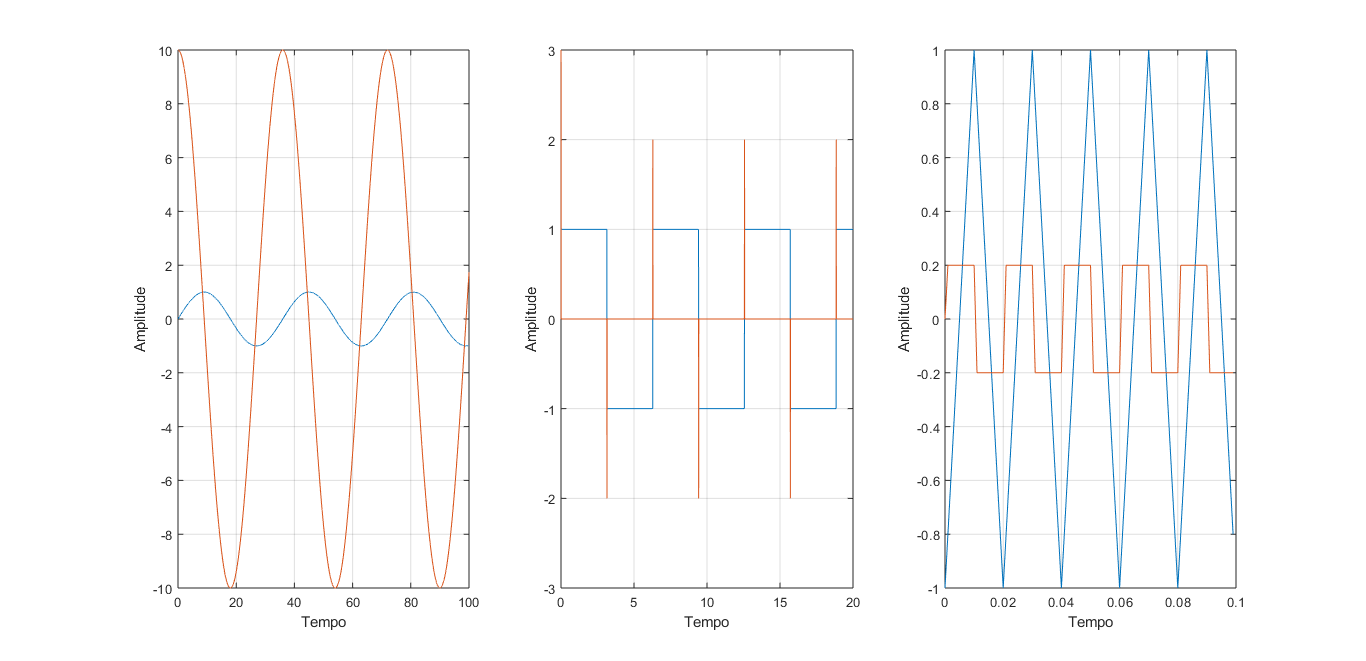
\includegraphics[width=1\textwidth]{imagens/plot_waves.png}
    \caption{Onda senoidal e sua derivada}
    \label{fig:onda_sin}
\end{figure}

% ---------------------------------------------------------------------

\subsubsection{Expressão em Laplace de $V_{out}(t)$ em função de $V_{in}$ do amplificador-diferenciador com $R_c=0$} 

Usando a expressão dada pela equação \ref{eqn:diff}, podemos escrever a transformada de Laplace como:


\begin{gather*}
	V_{out}(s) = -RC sV_{in}(s)
	\Longrightarrow \dfrac{V_{out}(s)}{V_{in}(s)} = H(s) = -RCs
\end{gather*}

Para analisar essa função de transferência, podemos plotar o diagrama de bode e observar seu comportamento.

\begin{figure}[H]
	\centering
	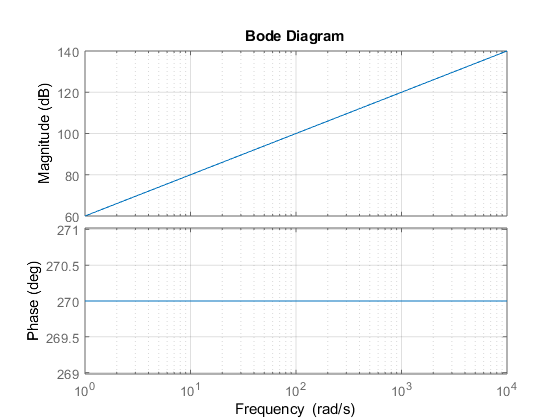
\includegraphics[width=.4\textwidth]{imagens/bode_plot.png}
	\caption{Diagrama de Bode da função de transferência}
	\label{fig: bode_dia}
\end{figure}

Considerando $R=1 k\Omega$ e $C=1F$, a função de transferência nos da um zero em 0 e um valor constante inicial de $20\cdot log(1000) = 60$. Como temos apenas um zero, a magnitude irá aumentar $ 20dB$ por década. Isso significa que quanto mais aumentarmos a frequência, maior será a amplitude da onda observada.
O que implica que, aumentando a tensão rapidamente, podemos chegar a um estado de saturação do Amp Op a partir de frequências muito pequenas dependendo do dimensionamento dos componentes.

\subsubsection{Expressão em Laplace de $V_{out}(t)$ em função de $V_{in}$ da Fig. \ref{fig:diferenciador} com $R_c>0$}

A forma mais simples de deteminar a função de transferência é transformando os componentes em impedâncias, como na figura abaixo:


\begin{figure}[H]

	\centering
	
    \begin{circuitikz}[line width = .5pt, scale = .8, transform shape]
        \draw
            (0,0) node [op amp] (opamp) {}
		
		(opamp.-) to [short] ($(opamp.-)+(0,1)$) to [generic, l_= $Z_2$]  ($(opamp.-)+(-2.8,1)$) to [generic, l_=$Z_1$] ($(opamp.-)+(-4,1)$) to [short, -o] ($(opamp.-)+(-5,1)$) node [left]{$V_{in}(t)$}
		(opamp.-) to [short, -*] ($(opamp.-)+(0,1)$)
		to [generic, l^=$Z_3$] ($(opamp.-)+(2,1)$) -| (opamp.out) to [short, *-o] ($(opamp.out)+(1,0)$)
		node [right] {$V_{out}(t)$}

		(opamp.+) to [short] ($(opamp.+)+(0,-1)$) node [ground]{}		
		;
		\draw ($(opamp.-)+(0,1)$)node[above] {A};
        
    \end{circuitikz}
    \caption{Circuito amplificador-diferenciador}
    \label{fig:diferenciador_imp}
\end{figure}


Fazendo as equações a partir da lei de Kirchhoff, obtemos:
\begin{gather*}
	\dfrac{V_A - V_{in}}{Z_1 + Z_2} + \dfrac{V_A -V_{out}}{Z_3} = 0
	\Longrightarrow\dfrac{V_{out}}{Z_3} = \dfrac{-V_{in}}{Z_1 + Z_2}\\
	\dfrac{V_{out}(s)}{V_{in}(s)} = H(s) = \dfrac{Z_3}{Z_1 + Z_2} 
\end{gather*}
Substituindo $Z_1 = R_c, \, Z_2 = \dfrac{1}{sC}, \, Z_3 = R$, temos
\begin{equation}
	H(s) = \dfrac{-RsC}{R_c sC + 1}
\end{equation}

Com uma rápida inspeção, podemos notar que a função tem um zero e um polo. O que significa que, em alguma frequência, o circuito irá se estabilizar. 

\begin{figure}[H]
	\centering
	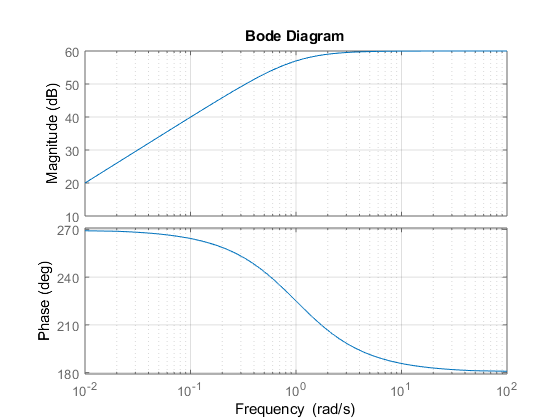
\includegraphics[width = .4\textwidth]{imagens/bode_plot_w_rc.png}
	\caption{Gráfico de Bode com $R_c>0$.}
\end{figure}

Observando o diagrama de bode dessa função de transferência com $R_c = 1\Omega, \, R = 1k\Omega \, e \, C = 1F$, podemos perceber que o circuito se estabiliza a partir das frequências de 1 kHz, com um ganho de 60 dB constantes. 

\subsubsection{Expressão para $V_{out}(t)$ da Fig. 2.2, em função de $V_{in}(t)$ e assumindo $R\rightarrow\infty$}

Utilizamos da equação \ref{eqn:int} para gerar a função no domínio da frequência a partir da Transformada de Laplace. Assim, temos
\begin{gather*}
	V_o(s) 	= -\dfrac{1}{RC} \cdot \dfrac{1}{s} \cdot V_{in}(s)
	\Longrightarrow \dfrac{V_o(s)}{V_{in}(s)} = -\dfrac{1}{RCs} 
\end{gather*}

\begin{equation}
	H(s)	=	 -\dfrac{1}{RCs}
\end{equation}

Podemos observar que a função possui apenas um polo. Dessa forma, dada uma frequência baixa, a tensão no capacitor pode ser superabundante a fim de danifica-lo. O gráfico de Bode abaixo ilustra bem a preocupação.

\begin{figure}[H]
	\centering
	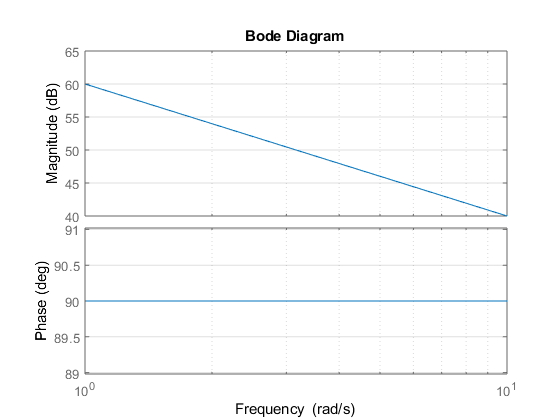
\includegraphics[width=.4\textwidth]{imagens/bode_plot_fig2_2_infty.png}
	\caption{Diagrama de Bode para $R_0 \rightarrow \infty$ }
	\label{fig: bode_2.2_rinf}
\end{figure}


Considerando C = $1\mu F$ e R = $1k\Omega$, temos uma ganho de 20 dB por década se decrescermos a frequência. Isso gera um risco para o capacitor ligado diretamente a saída do Amp Op. Por esse motivo, nunca devemos fazer $R_0 \rightarrow \infty$.

\subsubsection{Expressões para $V_{out}(t)$ da Fig. \ref{fig:integrador} em função de $V_{in}(t)$ assumindo $R_0$ finito}

Ilustrando o circuito no domínio da frequência, podemos realizar os cálculos usando apenas impedâncias, como ilustrado na figura \ref{fig:integrador_w_z}. Utilizando a Lei de Kirchhoff podemos obter a seguinte expressão.

\begin{gather*}
	\dfrac{V_A - V_{in}}{Z_1} + \dfrac{V_A-V_o}{Z_3} + \dfrac{V_A - V_o}{Z_2} = 0
	\Longrightarrow \dfrac{V_o(Z_3+Z_2)}{Z_3Z_2} = -\dfrac{V_{in}}{Z_1}
	\Longrightarrow \dfrac{V_o (s)}{V_{in}(s)} = H(s) = -\dfrac{Z_3Z_2}{(Z_3 +  Z_2)Z_1}
\end{gather*}

Substituindo $Z_3 = R_0, \, Z_2 = \frac{1}{sC}, \, e \, Z_1 = R$ e arranjando os termos, temos

\begin{equation}
	H(s) = -\dfrac{R_0}{R} \cdot\dfrac{1}{sR_0C + 1}
\end{equation}

\begin{figure}[H]
\centering
\begin{circuitikz}[line width = .5pt, scale = .8, transform shape]

\draw

	(0,0) node [op amp] (opamp) {}
	
	($(opamp.-)+(-3,1)$) node [left] {$V_{in}(t)$} 
	to [generic, l^= $Z_1$, o-*] ($(opamp.-)+(0,1)$) -| (opamp.-)
	
 	|- ($(opamp.-)+(0,1)$) coordinate (leftC) 
 	to [generic, l^=$Z_2$] (leftC -| opamp.out) -| (opamp.out)
 	to [short, *-o] ($(opamp.out)+(1,0)$) node [right] {$V_{out}(t)$}
 	
 	(opamp.+) to [short] ($(opamp.+)+(0,-1)$) node [ground] {} 
	;
	
	\draw   ($(opamp.-)+(0,1)$) -- ($(opamp.-)+(0,2.5)$); 
	\draw	($(opamp.-)+(0,2.5)$) to [generic, l^=$Z_3$] ($(opamp.-)+(2,2.5)$);
	\draw	($(opamp.-)+(2,2.5)$) -| (opamp.out){};
	\draw	($(opamp.-)+(0,0.8)$) node [left]{A};

\end{circuitikz}
	
	\caption{Circuito amplificador-integrador no domínio da frequência}
    \label{fig:integrador_w_z}
\end{figure}

Definindo $R_0 = 100 \Omega$, $R= 1k\Omega$ e C = $1\mu F$, podemos traçar o gráfico de bode dessa função de transferência para analisar seu comportamento.

\begin{figure}[H]
	\centering
	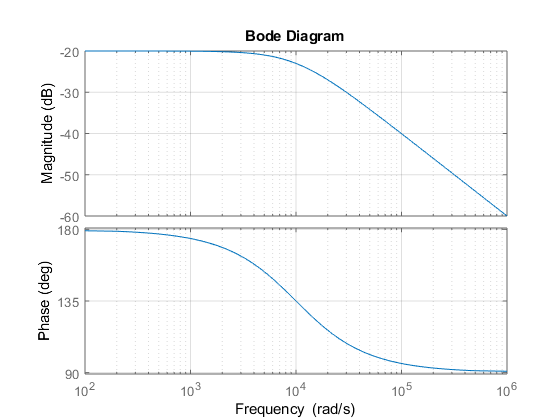
\includegraphics[width=.4\textwidth]{imagens/bode_plot_fig2_2_fty.png}
	\caption{Diagrama de Bode para $R_0$ finito}
	\label{fig:integrador_r0_fin}
\end{figure}

Esse circuito é conhecido como circuito integrador com limitação do ganho em D.C.

Observe que nos cálculos desprezamos o termo k, o qual resultaria na transformada $k=\frac{1}{s}$. A supressão foi feita a partir da hipótese de condição inicial nula. Deixaremos a cargo do leitor a análise do caso em que a condição inicial é não nula.

A inserção de $R_0$ resultou numa estabilidade do circuito antes de encontrarmos o primeiro polo. Note que há uma queda de tensão desde o início. Se quiséssemos uma queda de tensão inicial nula, deveríamos dimensionar $R_0$ para ser idêntico a R.


\newpage
\section{Simulações}

Considere os circuitos abaixo:

\begin{minipage}{.5\textwidth}
    \circuito{
        \draw
    
        (0,0) node [ground]{} to [short,-*] (0,0)
        to [short](-2,0) to [american voltage source, invert, -*](-2,3)
        node [above, color = red]{$V_f$}
        to [short] (2,3) node [above, color = red]{$V_R$} to [R, l=R, f>_=$i_R$,*-] (2,0)
        to [short] (0,0);
    }{Circuito A}{circ_a}
\end{minipage}
\begin{minipage}{.5\textwidth}
    \circuito{
    \draw
    
    (0,0) node [ground]{} to [short,-*] (0,0)
    to [short](-2,0) to [american voltage source, invert, -*](-2,3)
    node [above, color = red]{$V_f$}
    to [R, l^=$R_2$] (2,3) node [above, color = red]{$V_R$} to [R, l=$R$, f>_=$i_R$,*-] (2,0)
    to [short] (0,0);
    
}{Circuito B}{circ_B}    
\end{minipage}

\vspace{.2cm}
\noindent
\subsection{Para o circuito A, determine a tensão $V_R$ e a corrente $i_R$ esperadas sobre o resistor $R = 100\ohm$ para valores de tensão $V_f$
iguais a 3 V, 5 V e 10 V.}

\begin{itemize}
    \item Abra o QUCS, vá em Main Dock e crie um novo
    projeto.
\end{itemize}

\figuras{.4}{imagens/sim/new_project}{Criação de um novo projeto.}{new_project} 

\begin{itemize}
    \item Na aba Componentes, vá em componentes
    agrupados e coloque três resistores no esquemático.
    Vá em Fontes e coloque três fontes de tensão DC. Vá
    em Ponteiras e coloque três amperímetros.
\end{itemize}

\begin{figure}[H]
    \centering

    \subfiguras{.3}{.8}{imagens/sim/dc_source}{}{} 
    \subfiguras{.3}{.8}{imagens/sim/curr_prove}{}{} 
    \subfiguras{.3}{.8}{imagens/sim/res_ins}{}{} 
\end{figure}

\begin{itemize}
    \item Conecte os componentes sem esquecer da
    referência do terra e ajuste seus valores para os
    pedidos no exercício. Nomeie os nós para mediar a tensão $V_R$.
\end{itemize}
\figura{.6}{imagens/sim/label_item}
\figuras{.4}{imagens/sim/circuito1}{Cirucito a ser montado no Qucs}{circ_1}

\begin{itemize}
    \item Clique duas vezes na fonte de tensão. No valor de tensão insira o nome "Tensao" para que possa ser usado no parâmetro de varredura posteriormente.
\end{itemize}
\figuras{.4}{imagens/sim/nome_source}{Inserção da variável de varredura.}{var_sweep} 

\begin{itemize}
    \item Na aba simulações, insira a simulação DC e a simulação por varredura. 
\end{itemize}
\figuras{.3}{imagens/sim/ins_sim}{Inserção da simulação DC e da simulação por varredura.}{ins_sim1}

\begin{itemize}
    \item Configure as propriedades da simulação por varredura para o modo lista ("list"), o parâmetro de varredura ("Parameter Sweep") deve ser o mesmo atribuído à fonte de tensão, "Tensao". Os valores ("Values") devem ser 3V, 5V e 10V, como exigido pelo exercício.
\end{itemize}
\figuras{.4}{imagens/sim/swep_param}{Configuração dos parâmetros de varredura.}{} 

\begin{itemize}
    \item Salve e simule. Insira uma tabela para verificar os valores.
\end{itemize}
\figura{1}{imagens/sim/save_sim} 
\figuras{.3}{imagens/sim/ins_diagram}{Iserção de uma tabela.}{}

\begin{itemize}
    \item Insira os valores de $V_R$ e $i_R$ na tabela.
\end{itemize}
\figuras{.5}{imagens/sim/diagram_param}{Parâmetros da tabela.}{} 

\begin{itemize}
    \item Assim, verifica-se os valores exigidos pelo exercício.
\end{itemize}

\figuras{1}{imagens/sim/final1}{Resultado esperado pelo exercício.}{} 

\subsection{Repita os cálculos para o circuito B, considerando $R_2 = 50 \ohm$.}

\begin{itemize}
    \item Abra um novo esquemático.
\end{itemize}
\figuras{.5}{imagens/sim/new_sch}{Criação de um novo esquemático.}{} 

\begin{itemize}
    \item Na aba Componentes, vá em componentes
    agrupados e coloque seis resistores no esquemático.
    Vá em Fontes e coloque três fontes de tensão DC no
    esquemático. Vá em Ponteiras e coloque três
    amperímetros no esquemático.
\end{itemize}

\begin{figure}[H]
    \centering

    \subfiguras{.3}{.8}{imagens/sim/dc_source}{}{} 
    \subfiguras{.3}{.8}{imagens/sim/curr_prove}{}{} 
    \subfiguras{.3}{.8}{imagens/sim/res_ins}{}{} 
\end{figure}

\begin{itemize}
    \item Conecte os componentes sem esquecer da
    referência do terra e ajuste seus valores para os
    pedidos no exercício como na figura abaixo. Insira, também, um nome para o nó referente à $V_f$.
\end{itemize}

\figura{.5}{imagens/sim/label_item}
\figuras{.4}{imagens/sim/circuito2}{Circuito B a ser montado.}{}

\begin{itemize}
    \item Clique duas vezes na fonte de tensão. No valor de tensão insira o nome "Tensao" para que possa ser usado no parâmetro de varredura posteriormente.
\end{itemize}

\figuras{.5}{imagens/sim/nome_source}{Nomeação da variável de varredura.}{} 

\begin{itemize}
    \item Na aba simulações, insira a simulação DC e a simulação por varredura. 
\end{itemize}

\figuras{.3}{imagens/sim/ins_sim}{Inserção dos componentes de simulação.}{} 

\begin{itemize}
    \item Configure as propriedades da simulação por varredura para o modo lista ("list"), o parâmetro de varredura ("Parameter Sweep") deve ser o mesmo atribuído à fonte de tensão, "Tensao". Os valores ("Values") devem ser 3V, 5V e 10V, como exigido pelo exercício.
\end{itemize}

\figuras{.5}{imagens/sim/swep_param_2}{Parâmetros para a varredura.}{} 

\begin{itemize}
    \item Salve e simule. Insira uma tabela para verificar os valores.
\end{itemize}


\figura{1}{imagens/sim/save_sim}
\figuras{.3}{imagens/sim/ins_diagram}{Inserção de uma tabela.}{} 
\begin{itemize}
    \item Insira os valores de $V_R$ e $i_R$ na tabela.
\end{itemize}

\figuras{.5}{imagens/sim/diagram_param}{Configuração dos valores da tabela.}{} 

\begin{itemize}
    \item Assim, verifica-se os valores exigidos pelo exercício.
\end{itemize}

\figuras{1}{imagens/sim/final2}{Resultado esperado pelo exercício.}{} 

\newpage

\subsection{Ainda para o circuito B, faça $V_f = 10 V$ e calcule os valores de corrente fornecidos pela fonte se $R_2$ for um resistor de: $1 k\ohm$,
$500 \ohm$, $200 \ohm$, $100 \ohm$ e $50 \ohm$.}

\begin{itemize}
    \item Vá em Arquivo $\rightarrow$ Salvar como... e mude o nome do
    arquivo para utilizar o esquemático já montado para
    a segunda parte da simulação do Circuito B.

    \item Modifique a fonte de tensão para o valor de 10V, como mostrado abaixo.
\end{itemize}

\figuras{.4}{imagens/sim/circuito3}{Circuito a ser montado.}{}

\begin{itemize}
    \item Clique duas vezes no resistor $R_1$. Mude o valor de resistência para o nome "Resistor", como abaixo:
\end{itemize}

\figuras{.6}{imagens/sim/swep_var_res}{Definição da variável de varredura.}{}

\begin{itemize}
    \item Configure as propriedades da simulação por varredura para o modo lista ("list"), o parâmetro de varredura ("Parameter Sweep") deve ser o mesmo atribuído ao nome do resistor $R_1$, "Resistor". Os valores ("Values") devem ser 1 kOhm,
    500 ohm, 200 ohm, 100 ohm e 50 ohm, como exigido pelo exercício.
\end{itemize}

\figuras{.5}{imagens/sim/swep_param_3}{Configuração dos parâmetros da simulação por varredura.}{}


\begin{itemize}
    \item Salve e simule. Assim verifica-se os valores exigidos pelo exercício.
\end{itemize}

\figura{1}{imagens/sim/save_sim}
\figuras{.8}{imagens/sim/final3}{Resultado esperado pelo exercício.}{}



\end{document}